% !TeX root = ./tesi.tex
% !TeX encoding = UTF-8 Unicode
% !TeX spellcheck = it_IT
% !TeX program = arara
% !TeX options = --log --verbose --language=it "%DOC%"

% arara: lualatex:      { interaction: batchmode }
% arara: frontespizio:  { interaction: batchmode, engine: lualatex }
% arara: biber
% arara: lualatex:      { interaction: batchmode }
% arara: lualatex:      { interaction: nonstopmode, synctex: yes }

\documentclass[%
  a4paper,                % formato di pagina A4
  12pt,                   % corpo del testo a 12pt
  % la dimensione 12pt automaticamente imposta \footnotesize a 10pt
  twoside,                % (oneside|twoside) documento a singola o doppia facciata,
  openright,              % (openany|openright) fa cominciare un capitolo nella successiva pagina a disposizione o sempre in una pagina destra
  % twocolumn,            % dà a LaTeX le istruzioni per comporre l'intero documento su due colonne
  titlepage,              % (titlepage|notitlepage) se dopo il titolo del documento debbaavere  inizio  una  nuova  pagina
  % fleqn,                % allinea le formule a sinistra rispetto a un margine rientrato
  % leqno,                % mette la numerazione delle formule a sinistra anziché a destra
  final                   % (draft|final) scelta tra bozza o finale, influenza il comportamento degli altri pacchetti
]{scrbook}

\usepackage{fancyvrb}       % fornisce l'ambiente VerbatimOut e modifica listati di codice
% \usepackage{minted}       % evidenzia la sintassi dei listati di codice; richiede pygments installato e shell-escape

\begin{VerbatimOut}{\jobname.xmpdata}
\Title{Titolo}
\Subject{Oggetto}
\Author{Niccolò Maltoni}
\Copyright{Questo documento è fornito sotto licenza Apache License, Version 2.0}
\CopyrightURL{https://opensource.org/licenses/Apache-2.0}
\end{VerbatimOut}

\usepackage[%
  english,italian             % definizione delle lingue da usare
]{varioref}                     % introduce il comando \vref da usarsi nello stesso modo del comune \ref per i riferimenti

\usepackage[
  rgb,                        % richiesto da pdfx
  hyperref,                   % richiesto da pdfx
  luatex,
  dvipsnames,
  table,                      % permette di colorare le tabelle
  xcdraw
]{xcolor}                       % permette di usare colori
\usepackage[a-1b]{pdfx}         % permette di generare PDF/A
\usepackage{shellesc}           % aggiunge il comando \write18 necessario su Overleaf per frontespizio

%% Font
% non è necessario \usepackage[utf8]{inputenc} perché luaLaTeX accetta solo UTF-8
\usepackage{fontspec}
\setmainfont[%
  Ligatures=TeX               % abilita legature classiche di LaTeX
]{Latin Modern Roman}           % imposta il font con grazie per il testo principale
\setsansfont[%
  Ligatures=TeX               % abilita legature classiche di LaTeX
]{Latin Modern Sans}            % imposta il font senza grazie
\setmonofont[%
  Ligatures=TeX               % abilita legature classiche di LaTeX
]{Latin Modern Mono}            % imposta il font teletype monospaziato

%% Matematica
\usepackage{amsmath}
% non bisogna assolutamente invocare il pacchetto amssymb
\usepackage[%
  math-style=ISO              % per scrivere la matematica delle scienze sperimentali bisogna seguire le norme ISO
]{unicode-math}                 % implementazione di glifi Unicode per caratteri matematici
\setmathfont[%
  Ligatures=TeX               % abilita legature classiche di LaTeX
]{Latin Modern Math}
\usepackage[%
  output-decimal-marker={,},  % le convenzioni tipografiche italiane prevedono la virgola e non il punto
  binary-units                % abilita le espressioni per bit e byte
]{siunitx}                      % permette di definire numeri con unità di misura

%% Lingue
\usepackage[%
  strict=true,                % converte tutti i warning in errori
  autostyle=true,             % adatta continuamente lo stile delle virgolette alla lingua
  english=american,           % imposta lo stile per l'inglese
  italian=guillemets          % imposta lo stile per l'italiano
]{csquotes}                     % configura le virgolette secondo gli stnadard della lingua
\usepackage{polyglossia}
\setmainlanguage[%
  babelshorthands             % attiva il carattere " come switch per virgolettature etimologiche
]{italian}                      % imposta l'italiano come lingua principale
\setotherlanguage[%
  variant=american            % imposta la variante americana dell'inglese
]{english}                      % imposta l'inglese come lingua secondaria
% non è necessario \usepackage{indentfirst} perché con lualatex il rientro del primo capoverso è preimpostato

%% Altri pacchetti
\usepackage{graphicx}           % serve per includere immagini e grafici
\graphicspath{{res/fig}}      % importa la cartella res/fig/ come cartella da cui caricare le immagini
\usepackage{subcaption}         % serve per ottenere sottofigure
\usepackage{caption}            % permette di controllare la formattazione delle didascalie
\usepackage{adjustbox}          % permette di effettuare il crop delle immagini
\usepackage{xargs}
\usepackage[
  colorinlistoftodos,
  prependcaption,
  textsize=tiny
]{todonotes}                    % permette di definire note a margine di cose da fare
\newcommandx{\unsure}[2][1=]{\todo[linecolor=red,backgroundcolor=red!25,bordercolor=red,#1]{#2}}
\newcommandx{\change}[2][1=]{\todo[linecolor=blue,backgroundcolor=blue!25,bordercolor=blue,#1]{#2}}
\newcommandx{\info}[2][1=]{\todo[linecolor=OliveGreen,backgroundcolor=OliveGreen!25,bordercolor=OliveGreen,#1]{#2}}
\newcommandx{\improvement}[2][1=]{\todo[linecolor=Plum,backgroundcolor=Plum!25,bordercolor=Plum,#1]{#2}}
% \usepackage{ctable}           % permette di migliorare la spaziatura dell'ambiente tabular standard
% \usepackage{flafter}          % impedisce alle figure di apparire prima della loro definizione nel testo
\usepackage{scrhack}            % risolve incompatibilità tra KOMA e pacchatti vari (float, listings, ...)
\usepackage{float}              % permette di forzare il posizionamento dell’oggetto nel punto in cui è situato con l’opzione H
\usepackage{afterpage}          % permette di eseguire qualcosa nella pagina successiva con \afterpage{...} (ad esempio, figure)
% \usepackage{placeins}         % permette di mettere delle barriere invalicabili per le figure con \FloatBarrier
\usepackage[%
  write,                      % (write|nowrite) genera o meno il file
  standard,                   % (standard|suftesi) specifica tipo di frontespizio
  normal,                     % (normal|sans) usa font con grazie anziché senza
  noinputenc,                 % non carica inputenc (poiché usa lualatex)
  % norules,                  % non vengono inseriti filetti nel frontespizio
  nouppercase,                % con questa opzione verrà rispettato il maiuscolo e il minuscolo
  driver=luatex               % imposta la chiamata di graphicx nel documento frn per l'uso di un driver diverso da dvips o pdftex
]{frontespizio}
\usepackage{geometry}           % permettte la modifica della gabbia del documento
\geometry{
  a4paper,                    % formato di pagina
  heightrounded,              % modifica di poco le dimensioni della gabbia per contenere un numero intero di righe
  hmargin=2.5cm,              % dimensioni margini destro-sinistro
  vmargin=2.5cm               % dimensioni margini superiore-inferiore
}
\usepackage{setspace}           % serve a fornire comandi di interlinea standard
\onehalfspacing{}             % imposta interlinea a 1,5 ed equivale a \linespread{1,5}

%% Definizioni di comandi e ambienti
%% Definisco un nuovo comando per enfatizzare il testo in inglese %%%%%%%%%%%
\newcommand{\engEmph}[1] {\emph{\foreignlanguage{english}#1}}

%% Aggiunge pagine bianche vuote %%%%%%%%%%%%%%%%%%%%%%%%%%%%%%%%%%%%%%%%%%%%
\newcommand{\clearemptydoublepage}{\newpage{\pagestyle{empty}%
%\cleardoublepage}}
\clearpage}}

%% Definisce l'environment abstract per la classe book %%%%%%%%%%%%%%%%%%%%%%
\newenvironment{abstract}%
  {\cleardoublepage%
    \thispagestyle{empty}%
    \null\vfill\begin{center}%
      \bfseries\abstractname\end{center}}%
  {\vfill\null}

\usepackage[%
  maxcitenames=2,             % massimo numero di nomi nelle citazioni
  mincitenames=2,             % minimo numero di nomi nelle citazioni
  maxbibnames=99,             % massimo numero di nomi nella blibliografia
  minbibnames=99,             % minimo numero di nomi nella blibliografia
  style=ieee,                 % imposta lo stile della blibliografia (numeric|alphabetic|authoryear|authortitle|verbose|...)
  giveninits=true,
  backend=biber               % specifica il backend per la bibliografia
]{biblatex}                     % si interfaccia con bibtex e biber per la bibliografia
\addbibresource{biblio.bib}
\usepackage[%
  % page,                     % Aggiunge una pagina con la scritta Appendices
  % toc,                      % Aggiunge un campo Appendices nell'indice
  titletoc,                   % Aggiunge la parola Appendice per ogni capitolo dell'appendice nell'indice
  title%                      % Aggiunge la parola Appendice per ogni capitolo dell'appendice
]{appendix}                     % modifica la gestione dell'appendice, e aggiunge l'ambiente appendices alternativo al comando \appendix
% \usepackage[htt]{hyphenat}    % permette la sillabazione dei blocchi di testo monospaziato
% \usepackage{enumerate}        % aggiunge un argomento opzionale che determina come comporre l’etichetta numerata delle liste

\usepackage{microtype}          % gestisce la microtipografia

% \usepackage{hyperref}         % gestisce tutte le cose ipertestuali del pdf; importato automaticamente
\hypersetup{%
  pdfpagemode={UseNone},
  hidelinks,                  % nasconde i collegamenti (non vengono quadrettati)
  hypertexnames=false,
  linktoc=all,                % inserisce i link nell'indice
  unicode=true,               % usa solo caratteri Latini nei segnalibri di Acrobat
  pdftoolbar=false,           % nasconde la toolbar di Acrobat
  pdfmenubar=false,           % nasconde il menu di Acrobat
  plainpages=false,
  breaklinks,
  pdfstartview={Fit},
  pdflang={it}
}

\usepackage[%
  english,italian,            % definizione delle lingue da usare
  nameinlink                  % inserisce i link nei riferimenti
]{cleveref}                     % permette di usare riferimenti migliori dei \ref e dei varioref

\newcommand{\euler}{e}

\usepackage{tabularx}
\usepackage{listings}

\lstset{
  frame=tblr,
  tabsize = 4, %% set tab space width
  showstringspaces = false, %% prevent space marking in strings, string is defined as the text that is generally printed directly to the console
  numbers = left, %% display line numbers on the left
  commentstyle = \color{green}, %% set comment color
  keywordstyle = \color{blue}, %% set keyword color
  stringstyle = \color{red}, %% set string color
  rulecolor = \color{black}, %% set frame color to avoid being affected by text color
  basicstyle = \small \ttfamily, %% set listing font and size
  breaklines = true, %% enable line breaking
  numberstyle = \tiny,
}

\newcommand\blankpage{%
    \null
    \thispagestyle{empty}%
    \addtocounter{page}{-1}%
    \newpage}

\begin{document}

  \frontmatter{}
  \pagenumbering{Roman}
  \pagestyle{empty}
  % !TeX root = ../../tesi.tex
% !TeX encoding = UTF-8 Unicode
% !TeX spellcheck = it_IT

\begin{Preambolo*}
  \usepackage{fontspec}
  \setmainfont[Ligatures=TeX]{Latin Modern Roman}
\end{Preambolo*}
\begin{frontespizio}
  \Universita{Bologna}        % aggiunge da sé “Università degli Studi di”.
  \Istituzione{%
    Alma Mater Studiorum --- Università di Bologna \\%
    Campus di Cesena%
  }
  \Divisione{Dipartimento di Informatica --- Scienza e Ingegneria}
  \Corso[Laurea triennale]{Ingegneria e Scienze Informatiche}
  \Annoaccademico{2019--2020}
  \Titolo{DS4H Image Alignment: \\
  Modulo per allineamento multimodale semi-automatico considerando deformazioni solide}
  \Sottotitolo{Tesi in Programmazione}
  % \Preambolo{\renewcommand{\frontsmallfont}[1]{\small}}       % non viene stampata la matricola
  % \Preambolo{\renewcommand{\frontsmallfont}[1]{\small Matr.}} % abbrevia la matricola
  \Candidato[694493]{Marco~Edoardo~Duma}
  \NCandidato{Presentata da}  % sostituisce la parola “Candidato”
  \Relatore{Prof.~Antonella~Carbonaro}
  \Correlatore{Prof.~Filippo~Piccinini}
  \Correlatore{Prof.~Giovanni~Martinelli}
  \Piede{%                    % sostituisce la scritta “Anno Accademico” nel piede
    III sessione di laurea \\%
    Anno Accademico 2021--2022%
  }
\end{frontespizio}

% Necessario per Overleaf: compila il TeX del frontespizio subito dopo averlo generato
\IfFileExists{\jobname-frn.pdf}{}{%
\immediate\write18{lualatex \jobname-frn}}

  \blankpage
  % !TeX root = ../../tesi.tex
% !TeX encoding = UTF-8 Unicode
% !TeX spellcheck = it_IT

\clearemptydoublepage{}
\thispagestyle{empty}
\vspace*{20ex}
\begin{flushright}
    \begin{LARGE}
        \textbf{Parole chiave}\\
        \vspace{5ex}
    \end{LARGE}
    \begin{normalsize}
        \textbf{%
            Parola chiave 1\\%
            \medskip
            Parola chiave 2%
        }
    \end{normalsize}
\end{flushright}
\vfill

  \blankpage
  % % !TeX root = ../../tesi.tex
% !TeX encoding = UTF-8 Unicode
% !TeX spellcheck = it_IT

\clearemptydoublepage{}
\null{}\vspace{\stretch{1}}
\begin{flushright}
    \textit{Dedica}
\end{flushright}
\vspace{\stretch{2}}\null{}

  % !TeX root = ../../tesi.tex
% !TeX encoding = UTF-8 Unicode
% !TeX spellcheck = it_IT

\begin{abstract}
(EN) Most of the time, the deep analysis of a biological sample requires the acquisition of images at different time points, using different modalities and/or different stainings. These information give functional and morphological insights, but to really exploit the images acquired they must be co-registered to be then able to proceed with co-localisation analysis. Practically speaking, accordingly to the Aristotle’s principle “The whole is greater than the sum of its parts”, multi-modal image registration is the challenging task that brings to fuse together complementary signals. In the last years, several methods for image registration have been described in the literature, but unfortunately there is not one method that works for all applications. In addition, today there is no user-friendly tool for aligning images without any computer skills. In this work, besides revising all the solutions freely available for co-registering microscopy images, we describe DS4H Image Alignment, an open-source ImageJ/Fiji plugin for aligning multimodality, immunohistochemistry, and/or immunofluorescence 2D microscopy images, designed with the goal to be extremely easy-to-use.\hfill \break

\noindent (IT) Il più delle volte, l'analisi approfondita di un campione biologico richiede l'acquisizione di immagini in differenti momenti, utilizzando differenti modalità e/o colorazioni. Le informazioni acquisite forniscono dati funzionali e morfologici, ma per sfruttare realmente tutta la conoscenza, le immagini acquisite devono essere co-registrate per poter poi procedere con analisi di co-localizzazione. In pratica, secondo il principio aristotelico “Il tutto è maggiore della somma delle sue parti”, la registrazione multimodale dell'immagine è un compito impegnativo che porta a fondere insieme segnali complementari. Negli ultimi anni, sono stati descritti diversi metodi per la registrazione delle immagini, ma sfortunatamente non esiste un singolo metodo che funziona per tutte le applicazioni. Inoltre, oggi non esiste uno strumento intuitivo per l'allineamento delle immagini che non richieda importanti competenze informatiche da parte dell'utente. In questo lavoro, oltre a revisionare tutte le soluzioni disponibili gratuitamente per la co-registrazione di immagini di microscopia, descriviamo DS4H Image Alignment, un plug-in open source sviluppato per Fiji per l'allineamento di immagini 2D multimodali, di immunoistochimica e/o di immunofluorescenza, progettato con l'obiettivo di essere estremamente facile da utilizzare.
\end{abstract}

  \tableofcontents

  \mainmatter{}
  \pagenumbering{arabic}
  \pagestyle{headings}

  \chapter*{Introduzione}
    \noindent Il progetto di Tesi \textit{``DS4H Image Alignment''} è stato sviluppato all'interno del gruppo di ricerca \textit{``Data Science for Health''} (DS4H), gruppo che raccoglie professori e ricercatori del \textit{``IRCCS Istituto Romagnolo per lo Studio dei Tumori Dino Amadori''} (IRST) di Meldola (FC) e dell'\textit{Università di Bologna} (UniBo), professionisti attivi nel proporre metodi ed applicativi informatici per risolvere problemi aperti nel campo della microscopia e collegati al mondo della medicina, biologia e fisica. In particolare, per questo progetto di Tesi, la Prof.ssa Antonella Carbonaro e il Dr. Filippo Piccinini hanno sollevato il problema e proposto le prime soluzioni teoriche, e il Professore Giovanni Martinelli e il Professore Gastone Castellani hanno consentito l’acquisizione delle immagini utilizzate partendo dalla analisi di provini istologici di pazienti.\hfill \break
    \noindent \textit{DS4H Image Alignment} è un software nato con l’intento di fornire un applicativo estremamente user-friendly che permette ai ricercatori di allineare immagini 2D di provini istologici provenienti da pazienti, al fine di valutare con semplicità cross-correlazione tra differenti marcatori tumorali. Occorre specificare che ad IRST ogni giorno i medici, biologi, fisici analizzano provini istologici applicando differenti marcatori fluorescenti per individuare differenti caratteristiche tumorali. Da questi provini vengono tipicamente acquisite immagini, dove il soggetto di base è lo stesso (\textit{i.e.} il tessuto, la biopsia), ma l’oggetto marcato è differente (ad esempio, in alcune immagini possono essere usati dei marcatori per il nucleo delle cellule, in altre dei marcatori per la membrana, in altre dei marcatori per il citoplasma). È quindi utile poter disporre di uno strumento che riesca a fornire un'immagine unica che mostri allineate tutte le precedenti per poter apprezzare le caratteristiche del tessuto sovrapponendo le informazioni riportate nelle singole immagini precedentemente acquisite.\hfill \break
    \noindent Il progetto \textit{DS4H Image Alignment} è iniziato nel 2018 con la Tesi in Web Semantico di Stefano Belli~\cite{amslaurea19123}, poi diffusa attraverso l’articolo scientifico: \textit{J. Bulgarelli, M. Tazzari, A.M. Granato, L Ridolfi, S. Maiocchi, F. De Rosa, M. Petrini, E. Pancisi, G. Gentili, B. Vergani, F. PICCININI, A. CARBONARO, B.E. Leone, G. Foschi, V. Ancarani, M. Framarini, M. Guidoboni, Dendritic cell vaccination in metastatic melanoma turns “non-T cell inflamed” into “T-cell inflamed” tumors, Frontiers in Immunology, 2019. IF2019: 4.716. DOI: 10.3389/fimmu.2019.02353}.~\cite{Bulgarelli2019-oa} \hfill \break
    \noindent La prima versione di \textit{DS4H Image Alignment} prevedeva metodiche per l’allineamento manuale di immagini 2D di provini istologici. Le immagini facevano riferimento allo stesso provino ma erano relative a differenti marcatori fluorescenti. Per questo motivo il tool è stato descritto come un applicativo per registrazione multi-modale manuale. In pratica, \textit{DS4H Image Alignment 1.0} è in grado di gestire immagini di dimensione e scala differente, ma non presenta nessuna metodica per l’allineamento automatico. L’utente doveva definire punti di interesse corrispondenti in ciascuna immagine. Invece, la versione \textit{1.0} del software ha come obiettivo principale quello di limitare al massimo il numero di interventi a carico dell'utente e rendere il processo di allineamento delle immagini quanto più automatico possibile.\hfill \break
    \noindent Nei seguenti capitoli verrà descritto il contesto del progetto e verrà illustrata nei dettagli la soluzione proposta per l’allineamento multi-modale automatico. In particolare, nel \hyperref[chap:histology]{Capitolo 1} si dettagliano alcuni cenni di immunoistochimica per meglio comprendere la generazione di immagini multimodali utilizzando differenti marcatori fluorescenti. Nel \hyperref[chap:plugins]{Capitolo 2} si introduce l’ambiente di sviluppo e distribuzione del software, meglio definito come plugin/modulo. In particolare, è stato scelto di distribuire \textit{DS4H Image Alignment} come plugin di \textit{Fiji}, una versione specifica di \textit{ImageJ} molto diffusa tra i ricercatori. Nel \hyperref[chap:descriptionoldtool]{Capitolo 3} viene descritto in dettaglio \textit{DS4H Image Alignment}, in modo da riuscire a comprendere meglio quali sono le mancanze poi superate nella successiva versione. \textit{DS4H Image Alignment 1.0} è stato poi confrontato con i tool già presenti in letteratura, descritti nel \hyperref[chap:competitors]{Capitolo 4}. Infine, nel \hyperref[chap:descriptionnewtool]{Capitolo 5} viene descritto il modulo per l’allineamento multi-modale automatico cuore di questo progetto di Tesi, poi riassunto nel rimanente Capitolo.
  \chapter{Allineamento multi-modale per istologia}
\frenchspacing
\label{chap:histology}
\noindent L'istologia è il ramo delle discipline biologiche che studia la struttura microscopica e ultramicroscopica dei tessuti e degli organi animali e vegetali dal punto di vista morfologico, istochimico e delle attività funzionali da essi applicate~\cite{Istologia}.Tipicamente, si parte dalla analisi di un campione biologico o tessuto prelevato da paziente e tramite una sequenza di operazioni di preparazione si conducono analisi microscopiche per studiarne le caratteristiche normo-patologiche ed identificare malattie o problematiche in generale.
\section{Preparazione istologica}
La preparazione istologica è basata su 5 step fondamentali:
\begin{enumerate}
    \item Fissazione
    \item Disidratazione
    \item Inclusione
    \item Sezionamento
    \item Colorazione
\end{enumerate} \hfill \break
\noindent Il primo passo per produrre un campione istologico è quello della fissazione. Questa procedura è essenziale poiché comprende tecniche di conservazione del tessuto, tecniche atte a rafforzare la struttura cellulare ed infine una valutazione approfondita del campione per determinare se dev'essere esposto ad antigeni, in dipendenza dallo scopo per il quale è stato acquisito dello studio per il quale è stato acquisito~\cite{Alturkistani2015-bz}. \hfill \break
\noindent I fissativi più comuni sono a base di formaldeide, come ad esempio la formalina neutra tamponata (NBF) adoperata per preservare i tessuti o la paraffin-formalina (PFA) adoperata nel contesto dell'immunoistochimica.
A seguito della fissazione si procede con la disidratazione fatta tipicamente tramite etanolo, e la rimozione dell'alcol tramite xylene. Questa serie di operazioni serve a preparare i tessuti e rendere semplice la fase di sezionamento. \hfill \break
\noindent L'ultimo passaggio prima del sezionamento è quella dell'inclusione, che viene effettuata di solito tramite paraffina. Questo processo può portare ad un deterioramento delle cellule, a causa della prolungata esposizione al calore, e per evitare che ciò accada si congelano i tessuti dopo questa fase. \hfill \break
\noindent La fase di sezionamento concerne la preparazione di sezioni mediante microtomo. Le sezioni ottenute sono generalmente, molto sottili perché la luce dei microscopi possa passarci attraverso e permettere l'analisi da parte del ricercatore o specialista.
L'ultima fase è quella della colorazione ed andremo ad analizzarla in dettaglio nella prossima sezione.
\section{Co-registrazione multi-modale}
\noindent Durante la preparazione di un campione istologico vengono tipicamente usate più colorazioni per rivelare proprietà distinte del tessuto o di differenti componenti dello stesso. A causa dei lavaggi, e dei vari processi utili a completare ogni singola colorazione, il tessuto stesso viene però tipicamente deformato ed è richiesta quindi una registrazione non rigida delle varie immagini poi acquisite per poter procedere con una analisi globale del campione~\cite{9058666}.\hfill \break
\noindent Definiamo quindi con il termine ``registrazione multi-modale'' l'acquisizione e successivo allineamento di immagini provenienti dallo stesso campione ma che presentano delle differenze in termini di marcatura/colorazioni. Un esempio di queste marcature differenti è mostrato nelle \Cref{fig:1,fig:2,fig:3,fig:4} che rappresentano immagini, per la maggior parte acquisite in fluorescenza. L'immagine \Cref{fig:1} è stata colorata con Cy3, o Cianina, colorante visibile anche occhio nudo, che mette in evidenza il citoplasma della cellula.
Per la \Cref{fig:2}, è stato usato il DAPI, o ``4', 6-diamidin-2-fenilindolo'', è utile ad evidenziare i nuclei, per la \Cref{fig:3} il FITC, o Isotiocianato di fluoresceina, per le membrane ed infine \Cref{fig:4} usando la luce classica. \par
\noindent 
\begin{figure}[H]
    \centering
    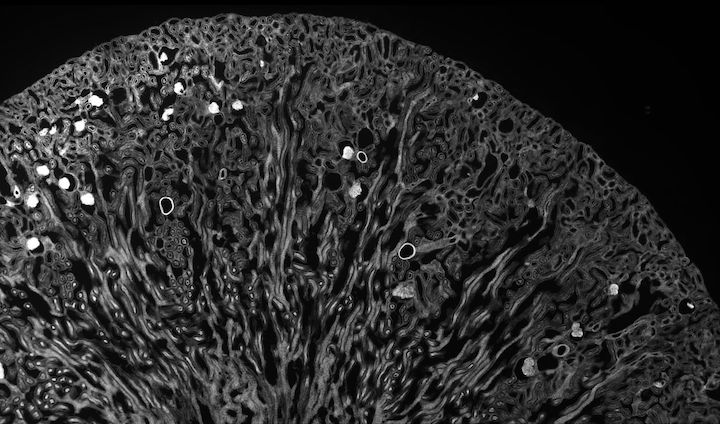
\includegraphics[scale=0.3,keepaspectratio]{multimodal/20190311_Mosaic_Cy3_NoAligned.jpg}
    \caption{Esempio di campione colorato con Cy3}
    \label{fig:1}
\end{figure}
\begin{figure}[H]
    \centering
    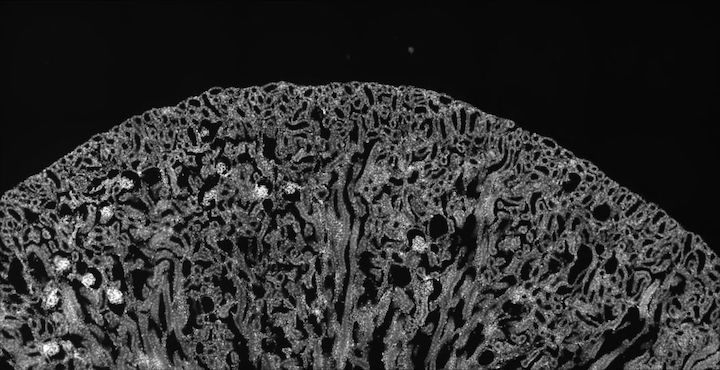
\includegraphics[scale=0.4,keepaspectratio]{multimodal/20190311_Mosaic_DAPI_NoAligned.jpg}
    \caption{Esempio di campione colorato con DAPI}
    \label{fig:2}
\end{figure}
\begin{figure}[H]
    \centering
    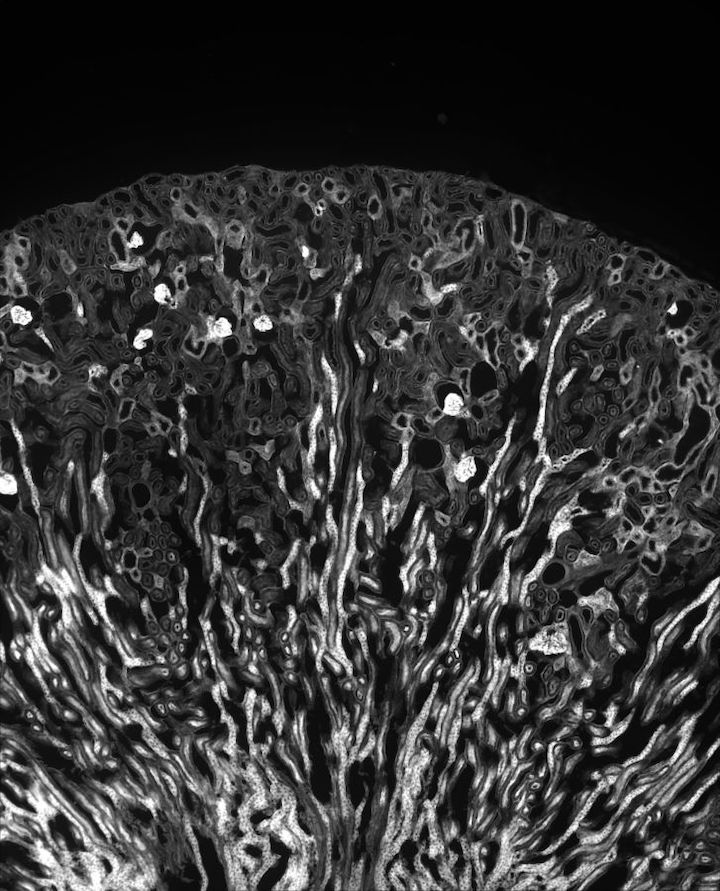
\includegraphics[scale=0.4,keepaspectratio]{multimodal/20190311_Mosaic_FITC_NoAligned.jpg}
    \caption{Esempio di campione colorato con FITC}
    \label{fig:3}
\end{figure}
\begin{figure}[H]
    \centering
    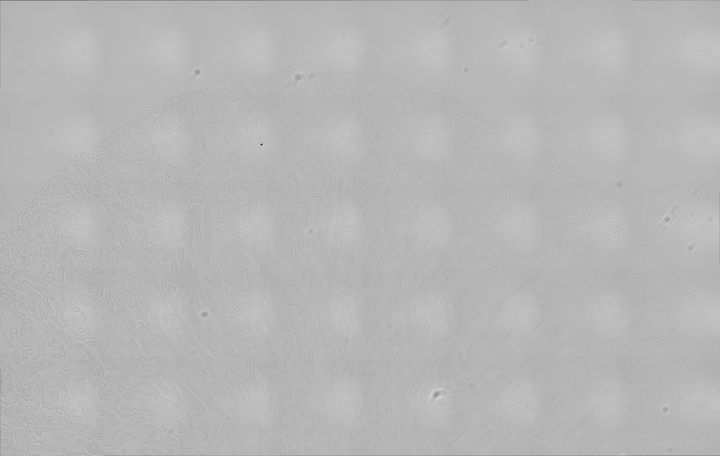
\includegraphics[scale=0.3,keepaspectratio]{multimodal/20190311_Mosaic_DICn2_NoAligned.jpg}
    \caption{Esempio di campione sottoposto a luce classica}
    \label{fig:4}
\end{figure}
\section{Algoritmi di co-registrazione automatica}
\noindent Per poter portare a compimento la co-registrazione multi-modale occorre utilizzare algoritmi di \textit{Computer Vision} in grado di occuparsi di questi cinque punti:
\begin{enumerate}
	\item Rilevamento delle caratteristiche salienti dell'immagine; 
	\item Definizione della corrispondenza delle caratteristiche tra diverse immagini;
	\item Rilevamento delle anomalie;
	\item Derivazione della funzione di trasformazione; 
	\item Ricostruzione dell'immagine finale.
\end{enumerate}
\noindent Chiariamo preventivamente che quando si utilizza il termine \textit{descrittore} si fa riferimento al contenitore che altro non è che il contenente di tutte le informazioni ottenute dopo l'elaborazione di un immagine. Di seguito descriveremo brevemente alcuni esempi di algoritmi noti per la registrazione di immagini, partendo da algoritmi, datati e dispendiosi in termini di risorse, fino a raggiungere quelli più recenti e performanti. \par
\subsection{SIFT - Scale Invariant Feature Transform}
\noindent L'algoritmo \textit{``SIFT''} (\textit{Scale Invariant Feature Transform}) è stato realizzato da D.G. Lowe nel 1999~\cite{Lowe2004}. Il rilevamento di corrispondenze tra immagini, è basato sull'algoritmo chiamato \textit{``Differenze di Gaussiane''}, abbreviato con l'acronimo DoG. Le DoG sono usate per trovare i punti d'interesse invarianti rispetto alla scala e all'orientamento. Per ogni agglomerato di punti si ricerca un modello adatto a determinarne posizione e scala, definendo punti chiave basati sulla stabilità delle loro misurazioni. Per ogni punto chiave viene assegnato un orientamento, in base alla direzione del gradiente locale dell'immagine. I gradienti locali delle immagini vengono misurati ad una scala selezionata, e vengono trasformati in una rappresentazione che permette di considerare cambi d'illuminazione e distorsione della forma.\hfill \break
\noindent La rappresentazione spazio-scala di un immagine è definita da una funzione L(x, y, \(\sigma\)) che è prodotta dalla convoluzione di una variabile spazio-scala Gaussiana G con un immagine in input I~\cite{Lowe2004}. \par
\begin{equation}
	L(x, y, \sigma) = G(x, y, \sigma) * I(x, y)
\end{equation}
\noindent dove la funzione G è definita da:
\begin{equation}
    G(x, y, \sigma) = \frac{1}{2\pi\sigma^2}\euler^\frac{-(x2+y2)}{2\sigma^2}
\end{equation}
\noindent
Al fine di individuare le collocazioni dei punti chiave stabili nella rappresentazione spazio-scala, esprimiamo una funzione D(x, y, \(\sigma\)) e calcoliamo la correlazione tra due scale vicine, facendo la differenza applicando al primo una costante moltiplicativa k:
\begin{equation}
	D(x, y, \sigma) = (G(x, y, k\sigma) - G(x, y, \sigma)) * I(x, y)
\end{equation}
\begin{equation}
    = L(x, y, k\sigma) - L(x, y, \sigma)
\end{equation}
\subsection{SURF - Speeded Up Robust Feature}
\noindent L'algoritmo \textit{``SURF''} (\textit{Speeded Up Robust Feature}) è nato nel 2006~\cite{BAY2008346}, come \textit{SIFT}, è basato sull'analisi della rappresentazione spazio-scala Gaussiana, ma si basa sul determinante dato da una matrice Hessiana. Grazie all'utilizzo di immagini integrali riesce a velocizzare il processo di identificazione di punti d'interesse. Questo lo rende, meno dispendioso a livello computazionale rispetto a SIFT.\hfill \break
\noindent Il concetto di immagine integrale espressa in forma matematica è data da I\(_{\Sigma}\) ad una posizione \textbf{x} = (x, y)\(^{T}\), ed è la somma di tutti i pixel presenti all'interno di una porzione rettangolare di un'immagine presa in input:
\begin{equation}
	I_{\Sigma} = \sum^{i \leq x}_{i=0} \sum^{i \leq y}_{j=0} I (i, j)
\end{equation}
\noindent Un Hessiana è una matrice quadrata le cui componenti sono derivate parziali seconde di una funzione, che nel caso di questo algoritmo ha questa forma:
\begin{equation}
	\begin{bmatrix}
		L_{xx}(\textbf{x}, \sigma) & L_{xy}(\textbf{x}, \sigma) \\
		L_{xy}(\textbf{x}, \sigma) & L_{yy}(\textbf{x}, \sigma)
	\end{bmatrix}
\end{equation}
\noindent Dove L\(_{**}\) è la convoluzione di una derivata seconda di una Gaussiana con l'immagine I nel punto \textbf{x}.
\subsection{BRISK - Robust Independent Elementary Features}
\noindent L'algoritmo \textit{``BRISK''} (\textit{Robust Independent Elementary Features}) è stato concepito nel 2011 da ricercatori dell'\textit{Autonomous System Lab} dell'Università \textit{ETH Zurich}~\cite{6126542}. Rispetto ai predecessori, il costo computazionale di questo algoritmo è molto ridotto. Tuttavia, ridotta è anche l'efficacia dell'algoritmo, ma dato l'enorme guadagno in termini di tempo, è generalmente considerato un prezzo accettabile.
\noindent Si compone di tre moduli principali~\cite{Liu2018-ds}: 
\begin{itemize}
	\item Individuazione dei punti chiave;
	\item Descrizione dei punti chiave; 
	\item Corrispondenza dei descrittori.
\end{itemize}
% primo modulo
\noindent Diversamente da \textit{SIFT} e \textit{SURF} che basano il riconoscimento di corrispondenza sulle regioni dell'immagini, questo algoritmo usa gli angoli delle immagini, che riconosce usando l'algoritmo AGAST (\textit{Adaptive and Generic Accelerated Segment Test})~\cite{10.1007/978-3-642-15552-9_14} e li filtra usando il punteggio restituito dall'algoritmo FAST (\textit{Features from Accelerated Segment Test})~\cite{Rosten2010-yf}. \hfill \break
% secondo modulo
\noindent La costruzione del descrittore di questo algoritmo è data dal pattern di campionamento, che stabilisce \textit{N} posizioni equidistanti in cerchi concentrici. Si definisce quindi un set A di coppie di punti dato da tutte le coppie di punti di campionamento:
\begin{equation}
	A = \{ (p_{i}, p_{j}) \in R^{2} \times R^{2} |\ i < B \wedge j < i, j \in \textit{N} \}
\end{equation}
\noindent Le coppie punti sono analizzate usando il rapporto che hanno in scala di grigi.
Per analizzare il gradiente locale tra i due punti \(p_{i}\) e \(p_{j}\), si prendono in considerazione i pixel smussati dai punti stessi annotandoli come \textit{I}(\(p_{i}\), \(\sigma_{i}\)) e \textit{I}(\(p_{j}\), \(\sigma_{j}\)). \par
\noindent L'analisi è data da:
\begin{equation}
	g(p_{i}, p_{j}) = (p_{i} - p_{j}) \cdot \frac{\textit{I}(p_{i}, \sigma_{i}) - \textit{I}(p_{j}, \sigma_{j})}{\|p_{j} - p_{i}\|}
\end{equation}
\noindent Dove i e j sono \(\geq\) 1 e \(\leq\) \textit{N}.\par
\noindent Detta \textit{t} la scala spaziale dei punti e \(\sigma_{max}\) e \(\sigma_{min}\) le soglie secondo cui definire due set S (breve distanza) e L (lunga distanza), abbiamo:
\begin{equation}
	S = \{ (P_{i}, P_{j}) \in A |\ \| P_{i} - P_{j} \| < \sigma_{max}\} \subseteq A
\end{equation}
\begin{equation}
	L = \{ (P_{i}, P_{j}) \in A |\ \| P_{i} - P_{j} \| < \sigma_{min}\} \subseteq A	
\end{equation}
\noindent La direzione complessiva del gradiente dei punti d'interesse viene stimato dal set \textit{L} come:
\begin{equation}
	g = \begin{bmatrix} g_{x} \\ g_{y} \end{bmatrix} = \frac{1}{l} \cdot \sum_{(p_{i}, p_{j}) \in L} g(p_{i}, p_{j})
\end{equation}
\noindent L'invarianza rispetto alla scala e alla rotazione è gestita tramite la rotazione dell'angolo \(\theta\) attorno al punto d'interesse k.
\begin{equation}
	\theta = {actan2} (g_{y}, g_{x})
\end{equation}
\noindent Per quanto riguarda invece l'intensità sulla breve distanza, definita nel set S, il descrittore viene prodotto da:
\begin{equation}
  b =
    \begin{cases}
      1 & \text{\(I(p_{j}^{\theta}, \sigma_{j}) > I(p_{i}^{\theta}, \sigma_{i})\)}  \\
      0 & \text{altrimenti}
    \end{cases}       
    \begin{tabular}{c}
      \text{\((P_{i}^{\theta}, P_{j}^{\theta}) \in S\)}
    \end{tabular}
\end{equation}
\noindent \(p_{i}^{\theta}\) rappresenta il punto \(p_{i}\) che ruota attorno al punto k ruotando \(\theta\). \hfill \break
\noindent La fase della corrispondenza delle caratteristiche, il cosiddetto \textit{Feature Matching}, si realizza tramite il confronto tra le somiglianze dei descrittori di due punti caratteristici. \par
\noindent Il Feature Matching è effettuato usando la distanza di Hamming per i descrittori binari, differentemente da \textit{SIFT} e \textit{SURF} che utilizzano le norme L1 o L2 per descrittori a base di stringhe. \par
\noindent Per misurare la distanza in maniera efficace vengono usate operazioni bit a bit XOR.
Ipotizzando di avere due descrittori \textit{X} e \textit{Y}, allora:
\begin{equation}
	X = \chi_{1}\chi_{2}\cdots\chi_{i}\cdots\chi_{N}
\end{equation}
\begin{equation}
    Y = \gamma_{1}\gamma_{2}\cdots\gamma_{i}\cdots\gamma_{N}
\end{equation}
\noindent dove il valore \(\chi_{i}\) e \(\gamma{i}\) può essere o 0 o 1. \par
\noindent L'equazione che esprime la distanza di Hamming è:
\begin{equation}
	HD(X, Y) = \sum_{i=1}^{N} \chi_{i} \oplus \gamma{i} = \sum_{i=1}^{n} b(\chi_{i}, \gamma{i})
\end{equation}
\noindent dove \(\oplus\) è lo XOR, e b(\(\chi_{i}, \gamma{i}\)) è l'espressione del i-esimo bit di X e Y:
\begin{equation}
	b(x, y) = \begin{cases}
      1 & \text{\( x \neq y \)} \\
      0 & \text{\( x = y \)}
    \end{cases}  
\end{equation}
\noindent In base al valore restituito dalla funzione HD si ha che più è alto, minore è il grado di corrispondenza tra descrittori.
\subsection{FREAK - Fast Retina Keypoint}
\noindent L'algoritmo \textit{``FREAK''} (\textit{Fast Retina Keypoint}) è stato proposto nel 2012~\cite{6247715}. È stato poi incluso in librerie di ``Computer Vision'' come \textit{``OpenCV''}, come alternativa agli algoritmi precedentemente descritti. Il fondamento della proposta è basato sulla topologia della retina umana, la quale compie in autonomia una codifica spaziale. L'algoritmo inizia usando una ``griglia a campionamento retinico''~\cite{6247715}, la quale si sviluppa in maniera circolare (\Cref{fig:5}), ha la particolarità di avere vicino al centro una densità maggiore di punti, e minore più ci si allontana da esso.
\begin{figure}[H]
    \centering
    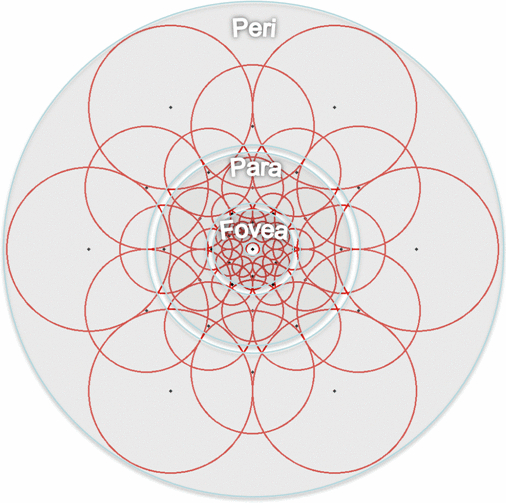
\includegraphics[scale=0.4,keepaspectratio]{circular-sampling-grid.jpg}
    \caption{Illustrazione del pattern di campionamento FREAK simile alla distribuzione delle cellule gangliari retiniche con i corrispondenti campi ricettivi. Ogni cerchio rappresenta un campo ricettivo in cui l'immagine viene levigata con il corrispondente kernel Gaussiano~\cite{6247715}}
    \label{fig:5}
\end{figure}
\noindent La sovrapposizione dei cerchi permette usare meno campi recettivi, poiché viene presa in considerazione come informazione da codificare, esattamente come per l'occhio umano che utilizza una strategia simile. Il descrittore binario, che per brevità chiameremo F, è costruito imponendo una soglia tra le coppie di campi recettivi e i loro Kernel Gaussiani (\ref{eq:1.18}) corrispondenti. \par
\begin{equation}
    {\displaystyle K(u)={\frac {1}{\sqrt {2\pi }}}e^{-{\frac {1}{2}}u^{2}}} \label{eq:1.18}
\end{equation}
\noindent Quindi ogni stringa binaria è composta da DoG rappresentati da un bit (\ref{eq:1.19}).
\begin{equation}
    F=\sum_{0\leq a < N}2^{a}T(P_{a}) \label{eq:1.19}
\end{equation}
\noindent dove \textit{\(P_{a}\)} è la coppia di campi recettivi e N la grandezza del descrittore desiderata e:
\begin{equation}
    T(P_{a})=\begin{cases}
       1 & \text{se \( (I(P_{a}^{r_{1}})-I(P_{a}^{r_{2}}) > 0 \)}  \\
       0 & \text{altrimenti}
    \end{cases}
\end{equation}
\noindent dove \textit{I} è l'intensità. Questa serie di operazioni porta ad avere un descrittore di una certa grandezza e per raffinarlo si seguono i seguenti passi:
\begin{enumerate}
    \item Dai punti corrispondenti estratti si crea una matrice D, in cui ogni riga rappresenta un punto chiave dato da tutte le possibili coppie. Si usano quindi 43 campi recettivi, questo porta ad avere approssimativamente 1000 coppie
    \item Per ogni colonna si calcola la media.
    \item Si ordinano le colonne rispetto alla varianza più alta.
    \item Prendiamo le colonne la cui media è di 0.5 e aggiungiamo a queste le rimanenti colonne che hanno una bassa correlazione con esse.
\end{enumerate}
\noindent Questo passaggio da grossolano a fine definisce la struttura del descrittore. Per mimare i movimenti individuali discontinui dell'occhio, si analizza in diversi step il descrittore. Si inizia l'analisi prendendo i primi 16 bytes che rappresentano l'informazione grossolana, e se la distanza è minore di una soglia si va avanti nella ricerca verso informazioni più fini.
Facendo così si accelera il processo di matching e si eliminano più del 90\% dei candidati.
Per calcolare la rotazione di un punto chiave, si sommano i gradienti locali stimati come nell'algoritmo BRISK.
\noindent Si prende un set \textit{G} di tutte le coppie usate per calcolare i gradienti locali:
\begin{equation}
    O=\frac{1}{M} \sum_{P_{o}\in G}(I(P_{o}^{r_{1}})-I(P_{o}^{r_{2}}))\frac{P_{o}^{r_{1}}-P_{o}^{r_{2}}}{\Vert P_{o}^{r_{1}}-P_{o}^{r_{2}}\Vert}
\end{equation}
\noindent dove M è il numero delle coppie dentro G a e \(P_{o}^{r_{i}}\) è il vettore delle coordinate spaziali in due dimensioni del centro del campo ricettivo.
  \chapter{Plugins per Fiji}
\label{chap:plugins}
\noindent Cosa è \textit{``Fiji''}? Come è nato? Quali sono le differenze con \textit{ImageJ} e come si sviluppa un plugin per l'applicativo preso in esame? Queste sono le principali domande a cui daremo risposta in questo capitolo.

\section{ImageJ}
\noindent \textit{``ImageJ''} è stato sviluppato nel 1997 dal \textit{NIH} (\textit{``National Institutes of Health''}). È un software open-source sostenuto da una vasta community di sviluppatori e ricercatori e oggi ed uno dei software più utilizzati da medici e biologi a fini scientifici.
È conosciuto all'interno della lista di distribuzioni ad esso collegate come \textit{``ImageJ 1.x''} o, per brevità IJ1. L'ultima versione risale al 31 marzo 2022 (\textit{1.53q}), ma al giorno d'oggi ancora attivo e ampiamente scaricato. È considerato un tool capace di adattarsi alla maggior parte dei problemi legati all'analisi di immagini, ed è per questo usato sia nel campo della microscopia che ad esempio in quello della scienza dei materiali. La libreria che lo compone è accessibile via API, permettendo a sviluppatori del settore di riusarne e estenderne le funzionalità attraverso la creazione di \textit{Plugin}, e di registrare \textit{Macro} automatizzando processi interni attraverso linguaggi come Java, Beanshell, Javascript e una DSL (\textit{Domain Specific Language}) per IJ1. L'utilizzo delle Macro permette ad utenti non Computer Scientists di non dover seguire un percorso di apprendimento particolare per l'automatizzazione di specifici workflow.

\section{Differenze tra ImageJ2 e ImageJ 1.x}
\noindent La seguente tabella è proveniente dalla fonte \cite{} e non è stata tradotta in lingua italiana per evitare incomprensioni.
\begin{table}[H]
\begin{tabularx}{\textwidth}{|l|X|X|}
\hline
\small{} &
\small{ImageJ 1.x} & 
\small{ImageJ2} \\
\hline
Image types & uint8, uint16, float32, rgb &	bit, uint2, uint4, uint8, uint12, uint16, uint32, uint64, uint128, int8, int16, int32, int64, float32, float64, cfloat32, cfloat64, bigint, bigdec, argb, <your-image-type-here> \\
\hline
Plugin types & PlugIn, PlugInFilter, PlugInTool & Command, Op, Tool, IOPlugin, Service, Converter, Codec, Format, DataHandle, TextFormat, ScriptLanguage, Display, UserInterface, Platform, App, Gateway, ModulePreprocessor, ModulePostprocessor, CodeRunner, ..., <your-plugin-type-here> \\
\hline
Dimensions & 5D—XYZCT &	N-dimensional—X, Y, Z, time, channel, emission spectra, lifetime, cell polarity, <your-dimension-here> \\
\hline
Image formats & HandleExtraFileTypes & SCIFIO—including Bio-Formats plugin; <your-format-here> \\
\hline
Parameters & GenericDialog & SciJava module @ parameter syntax—callable from ImageJ, KNIME, OMERO, CellProfiler, ..., <your-tool-here> \\
\hline
Script languages & IJ1 macro, JavaScript, BeanShell, Java &	BeanShell, Clojure (Lisp), Groovy, Java, JavaScript, JRuby, Jython (Python), Renjin (R), Scala, <your-language-here>\\
\hline
User interface & AWT & Legacy, Swing, AWT, Apache Pivot, Eclipse SWT, JavaFX, KNIME, CellProfiler, OMERO, <your-ui-here> \\
\hline
Distribution & Download, install and update manually & Hundreds of update sites; receive updates automatically (when you want!) \\
\hline
\end{tabularx}
\end{table}

\section{ImageJ2}
\noindent Il progetto \textit{``ImageJ2''} è nato nel 2009 ed è stato costruito su \textit{SciJava Common} che ne rappresenta il core. È il vero successore di \textit{ImageJ} 1.x. La libreria è stata infatti riscritta, ripensata e totalmente ridisegnata, facilitando l'estensibilità di tutti i tipi di dato. Segue i dettami dei principi \textit{SOLID} separando i compiti, disaccoppiando l'UI dal dominio applicativo, enfatizzando così la possibile integrazione con qualsiasi applicazione e/o libreria e portando il progetto ad essere interoperabile. Si può infatti intendere il progetto come un framework condiviso per l'elaborazione d'immagini attraverso il quale si può scrivere una sola volta il codice per eseguirlo su diversi applicativi come \textit{KNIME}, \textit{CellProfiler}, \textit{OMERO} e \textit{Icy}. La compatibilità verso la prima versione è una delle principali feature di cui dispone e ciò permette una facile migrazione agli sviluppatori tramite la libreria \textit{ImageJ Legacy}. È provvisto anche della libreria \textit{ImageJ Updater} per fare l'aggiornamento di ogni singolo plugin della libreria \textit{Imagej Ops} che comprende una serie di algoritmi di elaborazione immagini riusabili e di \textit{ImageJ Common} che usa \textit{``ImgLib2''} ed il core del modello dei dati delle immagini.
Infine per la maggior parte delle operazioni di I/O fa uso della libreria \textit{SCIFIO} (\textit{``SCientific Image Format Input and Output''}).


\section{Fiji}
\noindent È l'acronimo per \textit{Fiji is Just ImageJ}. L'architettura nasconde al suo interno la libreria \textit{ImageJ2} e fornisce un'estensiva lista di plugin forniti di default.
L'obiettivo principale di Fiji è migliorare l'esperienza utente dei ricercatori che non hanno conoscenze legate alla programmazione. I plugin forniti sono nella quasi totalità provvisti di una documentazione estensiva, dove si è guidati sia a livello generale con una prima panoramica delle funzionalità, sia a livello specifico in tutorial e dataset scaricabili. Il successo e la popolarità di \textit{Fiji} è dato anche dalla sua capacità di integrarsi per operazioni e compiti troppo onerosi per l'applicazione con applicativi terzi. \textit{Fiji} si interfaccia inoltre con MATLAB e \textit{ITK}, e attraverso \textit{ImgLib} e \textit{ImageJ2} e permette l'adozione di ogni piattaforma scritta in Java.


\section{Sviluppo di un plugin}

\subsection{Primi passi}
\noindent Prima di tutto si deve creare un progetto Java con un IDE a piacimento (\textit{``IntellJ IDEA''} o \textit{``Eclipse''} ad esempio) e creare un file pom.xml all'interno della radice del progetto. Per vedere un esempio pratico di questo osservare \textit{UnibosDS4H/DS4H} oppure \textit{imagej/example-imagej2-command}.

\begin{lstlisting}[language=XML,caption={Esempio parziale di file pom.xml UnibosDS4H/DS4H su Github}, label={lst:pom}]
<?xml version="1.0" encoding="UTF-8"?>
<project xmlns="http://maven.apache.org/POM/4.0.0"
...
<modelVersion>4.0.0</modelVersion>
<groupId>DS4H-Image-Alignment</groupId>
<artifactId>DS4H-Image-Alignment</artifactId>
<version>1.0.4</version>
<parent>
    <groupId>org.scijava</groupId>
    <artifactId>pom-scijava</artifactId>
    <version>25.0.0</version>
    <relativePath />
</parent>
<repositories>
    <repository>
        <id>imagej.public</id>
        <url>http://maven.imagej.net/content/groups/public</url>
    </repository>
</repositories>
    <dependencies>
        <dependency>
            <groupId>net.imagej</groupId>
            <artifactId>imagej</artifactId>
        </dependency>
    </dependencies>
</project>
\end{lstlisting}

\subsection{Il codice sorgente}
\noindent Si può scegliere di usare ImageJ2 o ImageJ 1.x, il quale viene tradotto automaticamente tramite un componente interno chiamato \textit{``Java Assist''}. Il primo esempio (\ref{lst:ImageJ2}) è quello consigliato al momento ed è la via preferibile, mentre il secondo esempio (\ref{lst:ImageJ1} e \ref{lst:ImageJ1Config}) è la versione Legacy che si può usare senza temere ma non permette di sfruttare le ultime features.

\begin{lstlisting}[language=Java,caption={Esempio semplice di un plugin Fiji in cui si fa uso di ImageJ2},label={lst:ImageJ2}]
package hello;

import org.scijava.command.Command;
import net.imagej.ImageJ;

@Plugin(type = Command.class)
public class HelloWorld implements Command {
	/**
	 * Main method is actually used only for debugging
	 **/
    public static void main(final String... args) {
        final ImageJ ij = new ImageJ();
        ij.launch(args);
        ij.command().run(HelloWorld.class, true);
    }
    @Override
    public void run() {
    	// ...
    }
}
\end{lstlisting}


\begin{lstlisting}[language=Java,caption={Esempio semplice di un plugin Fiji in cui viene utilizzato ImageJ 1.x}, label={lst:ImageJ1}]
package hello;

import ij.IJ;
import ij.plugin.PlugIn;

public class HelloWorld implements PlugIn {
    @Override
    public void run(String s) {
    	// ...
    }
}
\end{lstlisting}

\begin{lstlisting}[caption={Esempio di file plugins.config obbligatorio nel caso dell'uso di ImageJ 1.x}, label={lst:ImageJ1Config}]
	Plugins>Hello, "Hello World", hello.HelloWorld
\end{lstlisting}

\subsection{Transizione da ImageJ 1.x a ImageJ2}
\noindent Per chi ha già esperienza con la prima versione, qui può trovare una cheat sheet utile per effettuare la transizione alla seconda \Cref{fig:6} e \Cref{fig:7}.

\begin{figure}[H]
\centering
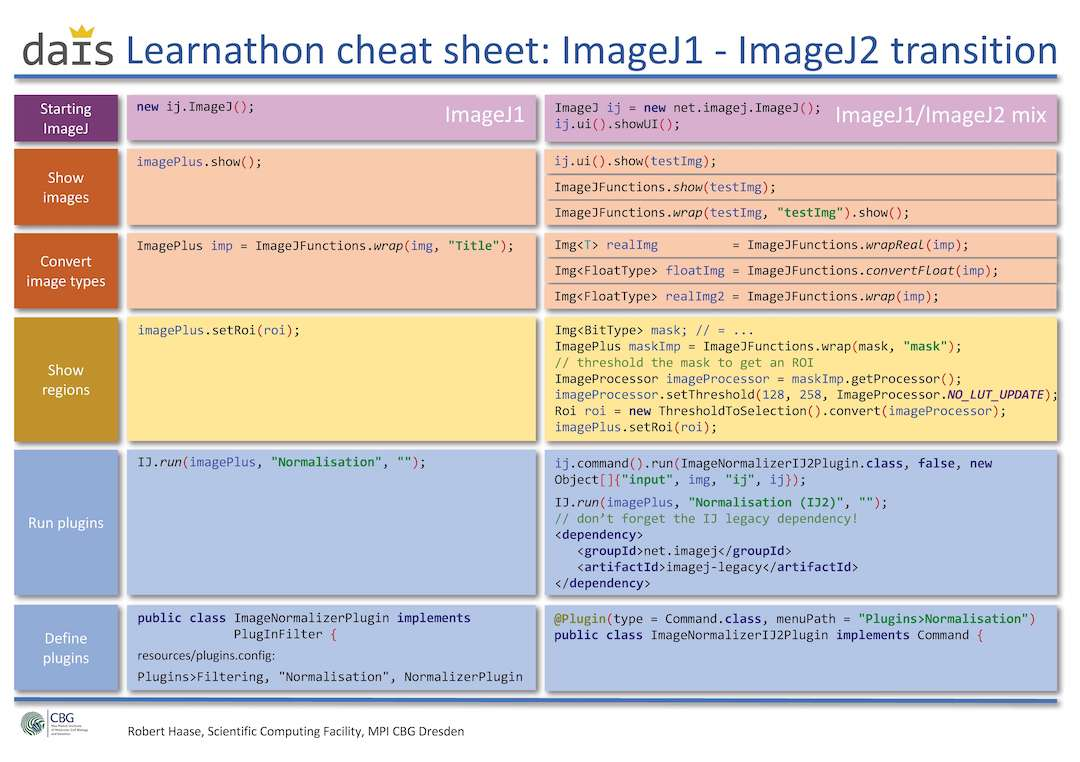
\includegraphics[scale=0.4,keepaspectratio]{ij_legacy_cheetsheet_Pagina_1.jpg}
\caption{Pagina 1, di Robert Haase, Scientific Computing Facility, MPI CBG Dresden}
\label{fig:6}
\end{figure}

\begin{figure}[H]
\centering
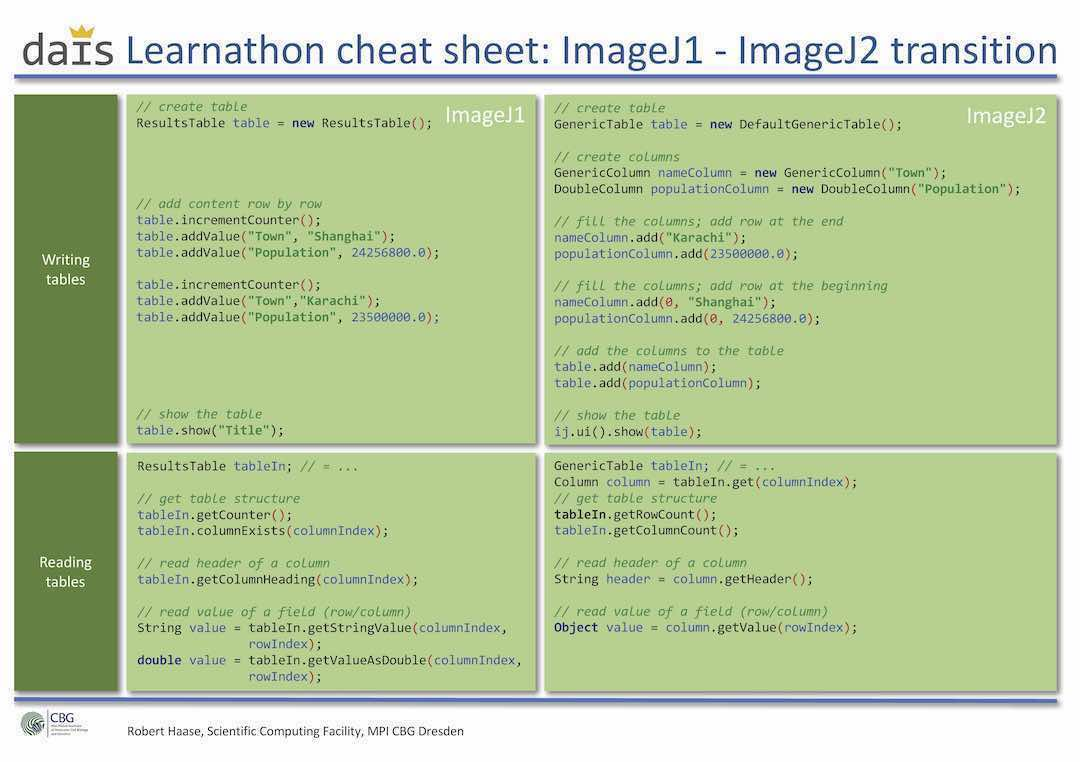
\includegraphics[scale=0.4,keepaspectratio]{ij_legacy_cheetsheet_Pagina_2.jpg}
\caption{Pagina 2, di Robert Haase, Scientific Computing Facility, MPI CBG Dresden}
\label{fig:7}
\end{figure}


\subsection{Build}
\noindent All'interno del file pom.xml dev'essere presente una parte di codice per eseguire il processo di creazione del file JAR, una di queste permette di includere agli assets \ref{lst:build}.

\begin{lstlisting}[language=XML, caption={"pom.xml, sottosezione build"}, label=lst:build]
<build>
	<resources>
        <resource>
            <directory>src/main/assets</directory>
            <includes>
                <include>**/*</include>
            </includes>
        </resource>
    </resources>
</build>
\end{lstlisting}

\noindent Per creare il file JAR nella giusta cartella occorre creare, se non già presente in questo percorso
\textbf{HOME/.m2}, un file chiamato \textbf{settings.xml} come mostrato in \ref{lst:scijavadir}

\begin{lstlisting}[language=XML, caption={"settings.xml valido per Fiji}, label={lst:scijavadir}]
<settings>
    <profiles>
        <profile>
            <id>imagej</id>
            <activation>
                <file>
                    <exists>${env.HOME}/Desktop/Fiji.app</exists>
                </file>
            </activation>
            <properties>
                <scijava.app.directory>${env.HOME}/Desktop/Fiji.app </scijava.app.directory>
            </properties>
        </profile>
    </profiles>
</settings>
\end{lstlisting}

\noindent Come compilare un file Maven dipende dall'IDE di riferimento. In questo paragrafo spiegheremo come si fa con \textit{IntellJ IDEA}, il quale fornisce tre modalità. La prima è tramite Run → Edit Configurations -> Maven, la quale non ha bisogno normalmente di specifici comandi per l'inizializzazione, e permette una volta eseguito di creare il file JAR. La seconda modalità è attraverso il plugin stesso, mostrato in \Cref{fig:8}, dove l'UI permette agli utenti meno esperti di usufruire dei comandi e dei profili Maven senza avere conoscenze pregresse.

\begin{figure}[H]
    \centering
    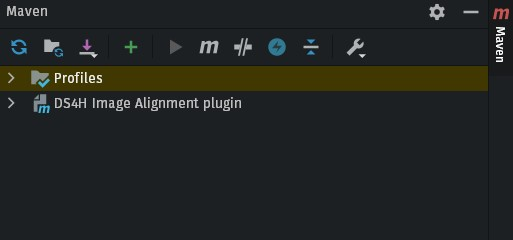
\includegraphics[scale=1,keepaspectratio]{plugin_maven_idea.jpg}
    \caption{Esempio plugin Maven IntelJ IDEA}
    \label{fig:8}
\end{figure}

\noindent L'ultima modalità è quella di digitare i comandi specifici direttamente dal terminale, ad esempio \ref{lst:mvn}:
\begin{lstlisting}[label={lst:mvn}, caption={Esempio per pulire, compilare e creare il file JAR}]
    mvn clean & mvn compile & mvn install
\end{lstlisting}

\subsection{Service}
\noindent A differenza di \textit{ImageJ 1.x}, dove per accedere alla maggior parte delle sue funzionalità si usano dei metodi statici, per \textit{ImageJ2} ogni parte ha la sua logica di business incapsulata in un servizio. Un servizio non è altro che una classe con una serie di responsabilità legate ad un solo argomento. \textit{ImageJ2} dispone di tantissimi Service, tra questi possiamo ricordare:
\begin{itemize}
    \item AppService - tiene traccia l'applicazione presente nel contesto.
    \item DisplayService - tiene traccia delle schermate disponibili, di quella attiva, e da l'abilità di crearne di nuove.
    \item EventService - gestisce gli eventi legati all'applicazione, ed è la base per gestire la comunicazione tra le diverse parti dell'applicativo.
    \item IOService - contiene gli strumenti per aprire e salvare file all'interno del contesto.
    \item MenuService - ha la struttura del menu dell'app che può essere costruita attraverso questo servizio.
    \item ModuleService - tiene traccia dei moduli disponibili, e fornisce l'infrastruttura per eseguirli.
    \item ObjectService - tiene traccia degli oggetti disponibili, inclusi i Datasets e i Displays.
    \item OptionsService - ha gli strumenti per gestire le impostazioni del programma.
    \item PlatformService - provvede hooks per estendere l'applicativo rispetto al sistema operativo in uso.
    \item PluginService - tiene traccia dei plugins, e fornisce gli strumenti per eseguirli.
    \item ScriptService - permette di eseguire gli script e macro.
    \item StatusService - tiene traccia dello stato delle operazioni in corso.
    \item ThreadService - gestisce multithreading, utile per eseguire più operazioni e task in parallelo.
    \item UIService - esegue le UI per interagire con ImageJ.
    \item DatasetService - ha gli strumenti per creare e gestire i dati delle immagini.
    \item ImageDisplayService - simile a DisplayService, ma per gli ImageDisplays.
    \item OverlayService - ha gli strumenti per creare e gestire gli overlays e le ROIs delle immagini.
    \item FormatService - servizio per gestire i formati delle immagini disponibili.
\end{itemize}
    


\subsection{Consigli}
\noindent La fase più importante per la creazione di software è la quella di progettazione del dominio e della business logic. È importante non pensare alle librerie che si useranno, poiché rappresentano una parte terza che dev'essere sempre possibile cambiare, ad esempio se si sceglie una differente libreria di UI durante la fase di sviluppo rispetto a quella già implementata, la modifica si deve poter fare senza dover cambiare parti del dominio. È buona pratica studiare il linguaggio usato, conoscere cosa si intende per OOP e cosa sono i principi SOLID.
  \chapter{Descrizione del DS4H Image Alignment Tool}
\label{chap:descriptionoldtool}
\noindent Il capitolo corrente descrive la prima versione del plugin \textit{DS4H Image Alignment}, progetto sviluppato da Stefano Belli nel 2019 come Tesi Magistrale in questo corso di studi.

\subsection{Struttura generale}
\noindent Il plugin ha una interfaccia utente organizzata in finestre modali. Le principali sono:
\begin{itemize}
	\item MainDialog - è la finestra incaricata di mostrare l’immagine corrente. Permette di aggiungere corners per l’allineamento manuale, e da accesso a tutte le altre finestre di dialogo del software.
	\item PreviewDialog - mostra una anteprima delle immagini riportando la lista delle coordinate dei corners già inseriti.
	\item RemoveDialog - permette di rimuovere le immagini precedentemente caricate.
	\item AlignDialog - finestra che mostra il risultato della co-registrazione delle immagini tramite corners, permette di salvare il risultato in file TIFF o di riutilizzare le stesse immagini per un nuovo ciclo di co-registrazione.
\end{itemize}

\noindent Le interazioni con l’utente vengono gestite dalla classe ImageAlignment, allaquale vengono comunicate le operazioni eseguite dalle finestre di dialogo tramite ActionListeners. Le immagini all’interno di \textit{ImageJ} sono incapsulate attraverso la classe ImagePlus, questo garantisce compatibilità con il framework SciJava. Per gestire le immagini viene usata una classe chiamata ImagesManager, che permette di scorrere le immagini caricate da parte dell’utente, reso possibile tramite l’implementazione dell’interfaccia ListIterator.
Le immagini sono racchiuse all’interno di BufferedImage che ne gestisce la visualizzazione; ogni immagine è racchiusa all’interno di una collezione chiamata ImageFile che permette l’estrazione metadati tramite la libreria bio-formats e restituisce il numero di immagini, la dimensione massima, la lista dei corner points registrati tramite ROIManager, etc.
Come si può notare dallo schema in \Cref{fig:9}, ogni istanza di BufferedImage viene generata a richiesta del rispettivo ImageFile per ridurre in maniera efficiente l’utilizzo della memoria.

\begin{figure}[H]
    \centering
    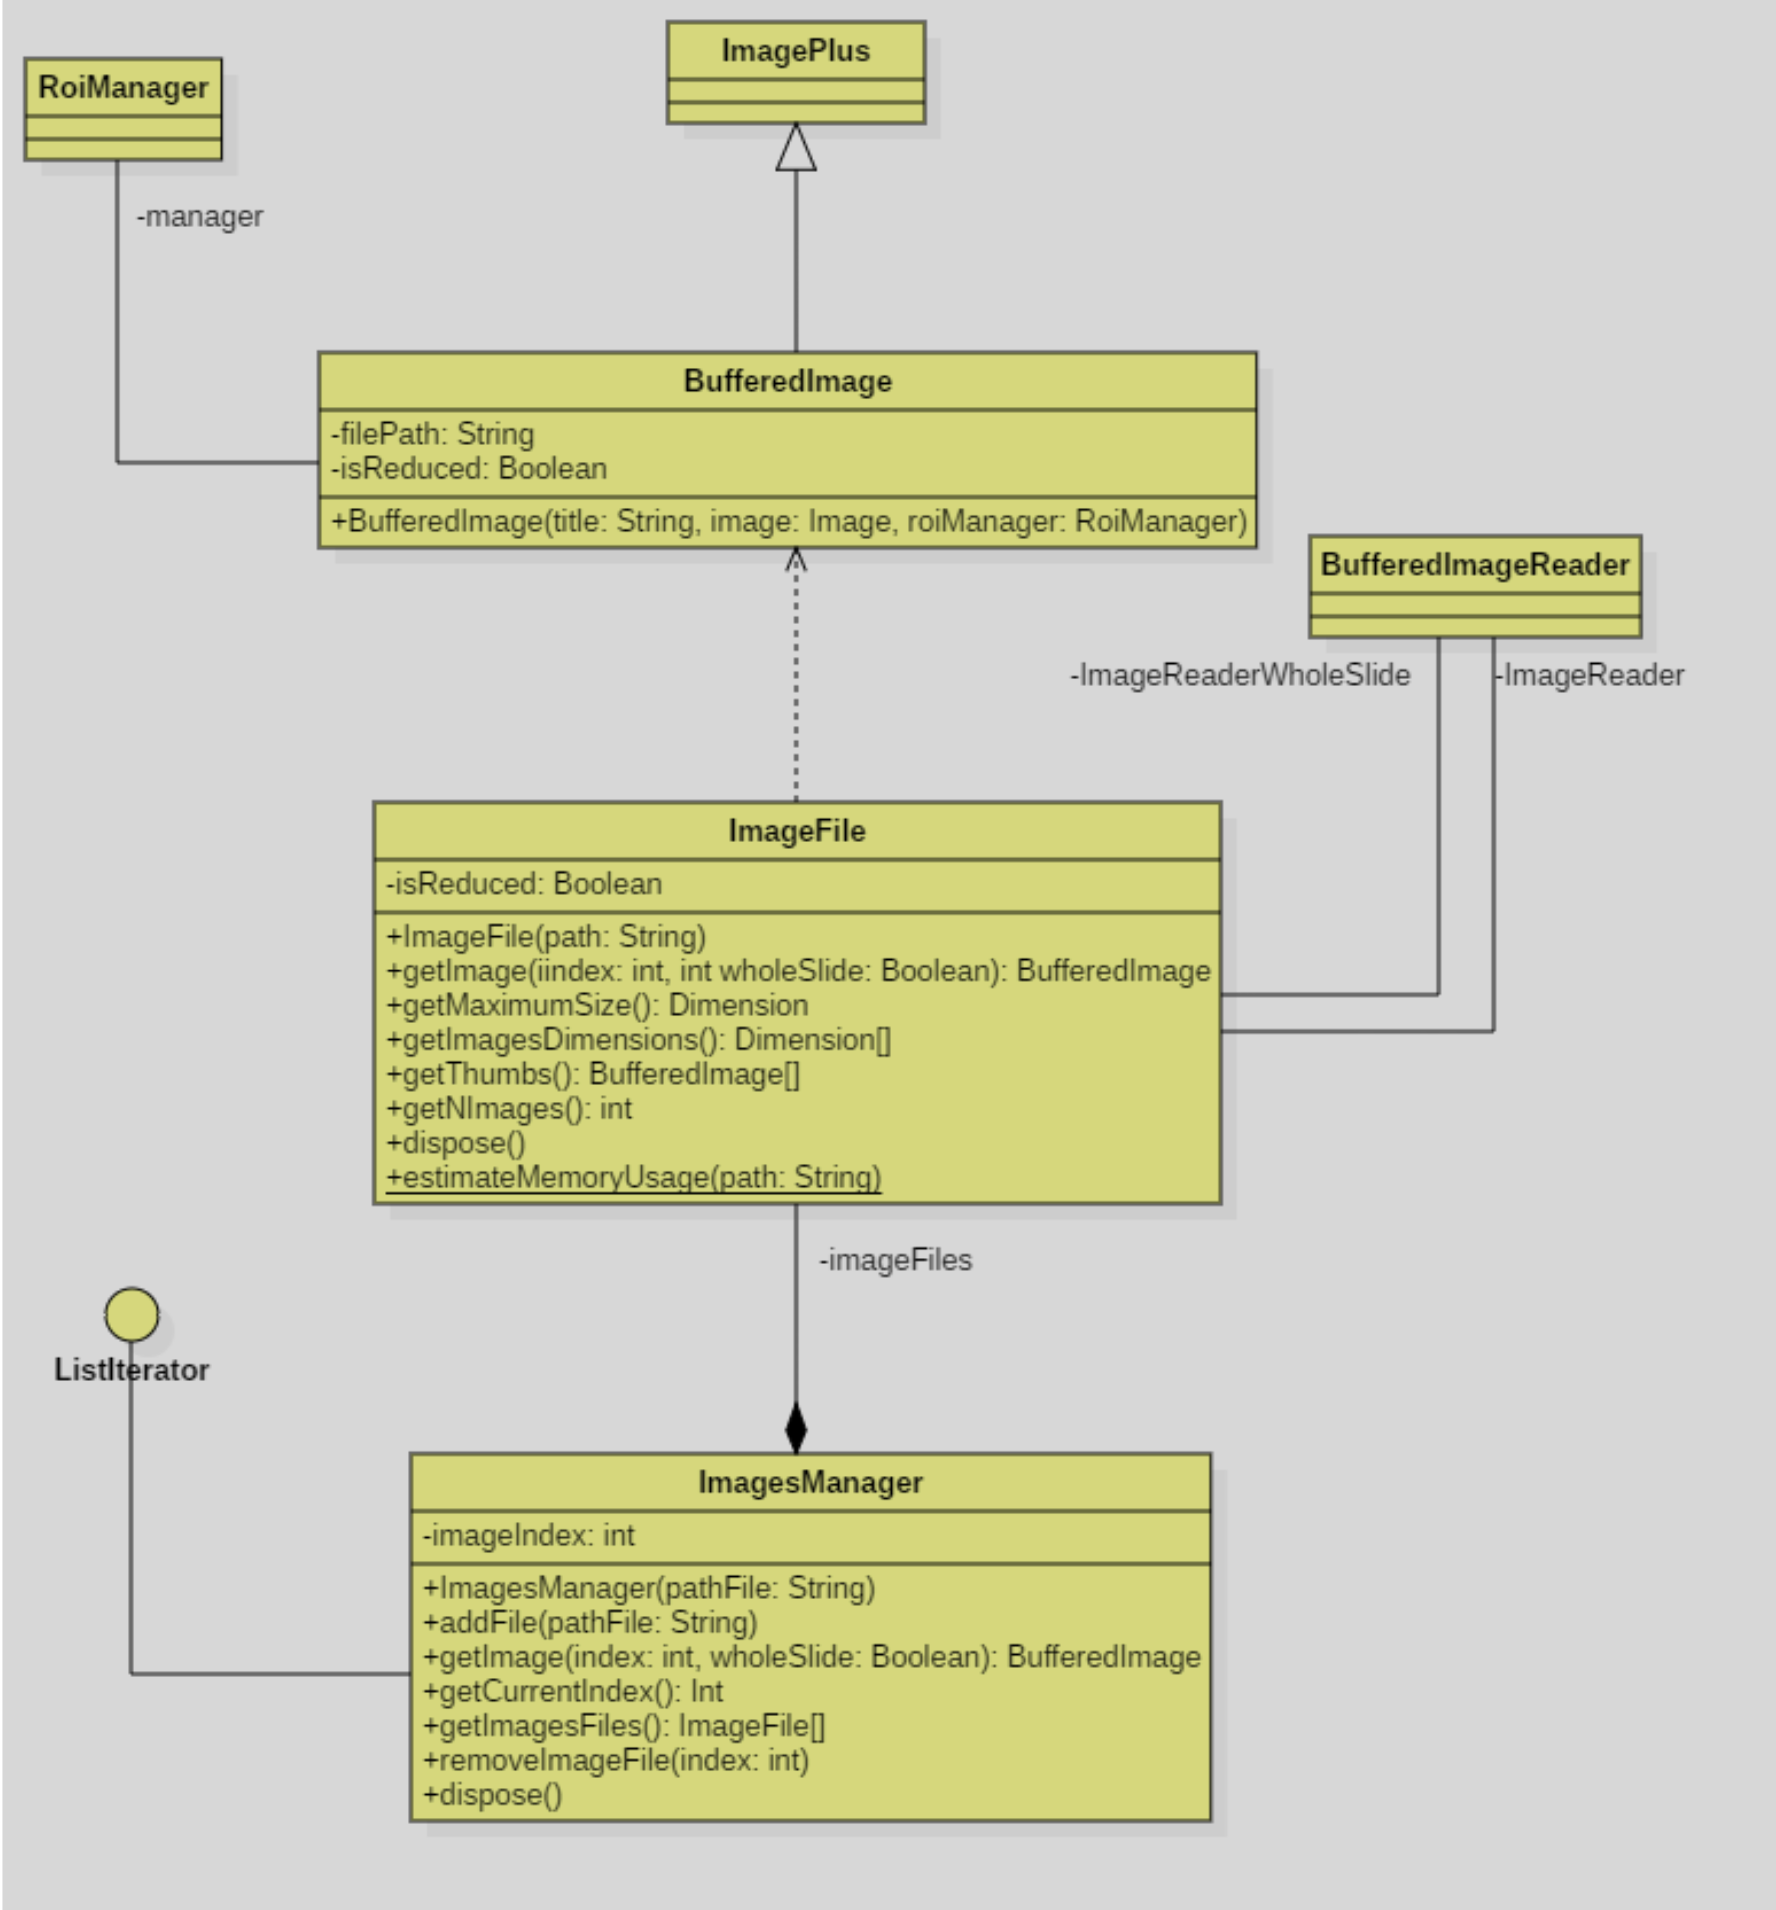
\includegraphics[scale=0.4,keepaspectratio]{SchemaImagePlus.png}
    \caption{Diagramma UML delle classi dati principali di DS4H}
    \label{fig:9}
\end{figure}


\subsection{Modalità d'uso dell'applicazione DS4H}
\noindent Di seguito sono spiegate tutte le funzionalità che il team di sviluppo ha provveduto a rendere disponibili all'utente.
Le schermate presentate in questa sezione provengono da un Macbook Pro M1 Pro.

\subsubsection{Aggiunta Corner Point}
\noindent Basta premere il tasto \textbf{C} all'interno dei limiti dell'immagine corrente, e rispettivamente al punto in cui si è premuto il tasto si mostrera un corner point.
L'esempio in \Cref{fig:10} mostra il risultato dell'operazione, dove si è premuto tre volte, e da cui si può notare l'ordine grazie alla numerazione.
\begin{figure}[H]
    \centering
    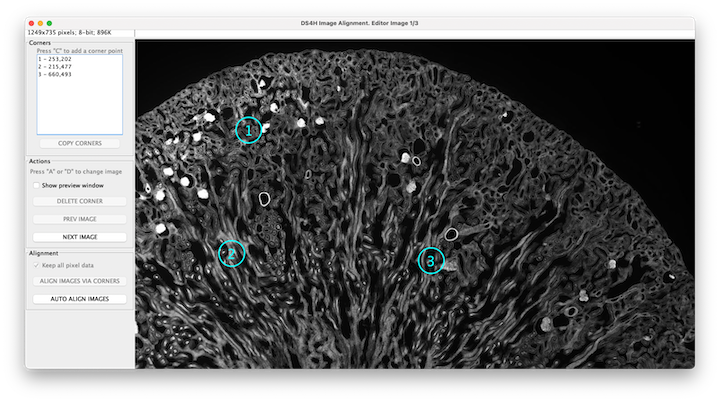
\includegraphics[scale=0.5,keepaspectratio]{windows/aggiunta_corner.png}
    \caption{Schermata principale in cui sono stati aggiunti dei corner points}
    \label{fig:10}
\end{figure}

\subsubsection{Modifica Corner Point}
\noindent Ogni corners point è modificabile nella sua forma trascinandolo tramite cursore come in \Cref{fig:11}.
\begin{figure}[H]
    \centering
    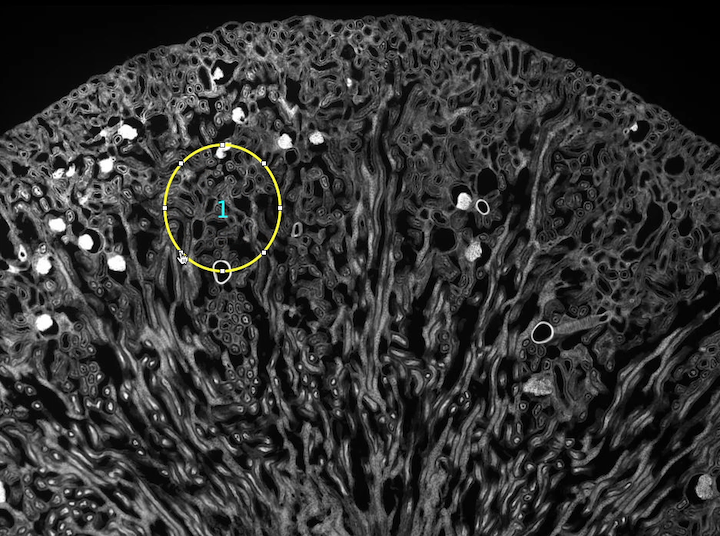
\includegraphics[scale=0.5,keepaspectratio]{windows/modifica_corner.png}
    \caption{Immagine corrente in cui sta venendo modificato un corner}
    \label{fig:11}
\end{figure}

\subsubsection{Rimozione Corner Point}
\noindent Ogni corner point una volta registrato è visibile e selezionabile anche attraverso una lista nella parte sinistra della finestra principale, ed una volta selezionato tramite cursore si può cancellare premendo il bottone in \Cref{fig:12} (``Delete Corner'').

\subsubsection{Cambia Image Corrente}
\noindent I botttoni ``Next Image'' e ``Prev Image'' in \Cref{fig:12} se premuti permettono di navigare tra le immagini importate.

\begin{figure}[H]
    \centering
    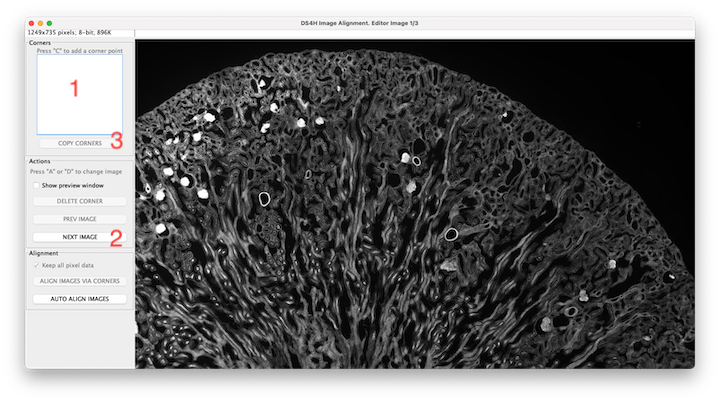
\includegraphics[scale=0.5,keepaspectratio]{windows/schermata_principale.png}
    \caption{Schermata principale i cui numeri definiscono: 1 Rimozione Corner, 2 Cambia Immagine, 3 Copia Corner}
    \label{fig:12}
\end{figure}

\subsubsection{Copia Corner Points}
\noindent Per facilitare l'apposizione dei corners in tutte le immagini l'applicazione è fornita di un bottone apposito visibile in \Cref{fig:12} che se premuto mostra una finestra di dialogo, come quello mostrato in \Cref{fig:13}. Da questa finestra è possibile scegliere l'immagine da cui importare i corner points, e nel caso in cui i corner points importati risultino fuori dai limiti delle immagini il sistema notifica l'utente di ciò, dando la possibilità di cancellare anche dall'immagine sorgente i suddetti punti \Cref{fig:14}.

\begin{figure}[H]
    \centering
    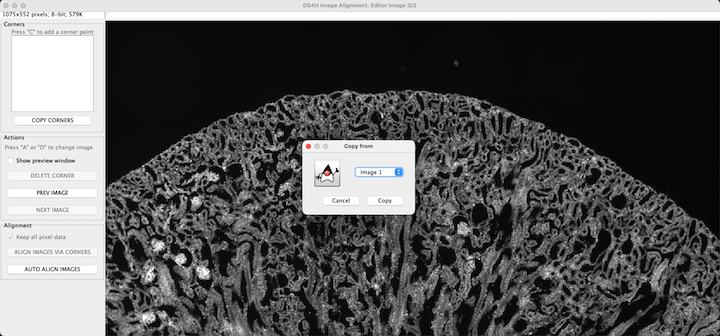
\includegraphics[scale=0.5,keepaspectratio]{windows/copy_corner_from_source.png}
    \caption{Finestra di dialogo da cui si può scegliere l'immagine sorgente per eseguire la copiatura}
    \label{fig:13}
\end{figure}

\begin{figure}[H]
    \centering
    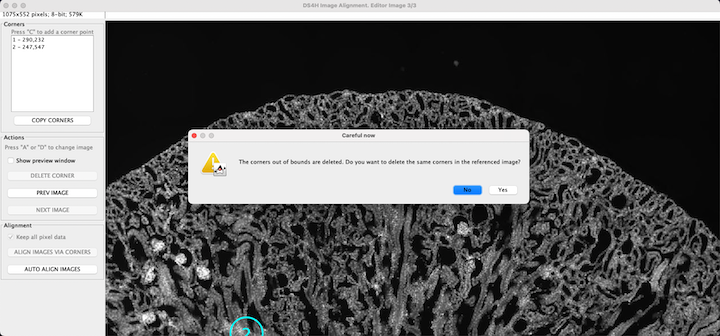
\includegraphics[scale=0.5,keepaspectratio]{windows/copy_corner_warning.png}
    \caption{Finestra di warning che notifica l'utente la presenza di corners fuori dai limiti dell'immagine}
    \label{fig:14}
\end{figure}

\subsubsection{Aggiunge e Rimuove File}
\noindent Dalla finestra principale, accedendo al menu ``File'' si possono eseguire sia l'importazione di una nuova immagine da aggiungere alla presente lista di immagini, sia rimuovere un immagine a scelta.

\begin{figure}[H]
    \centering
    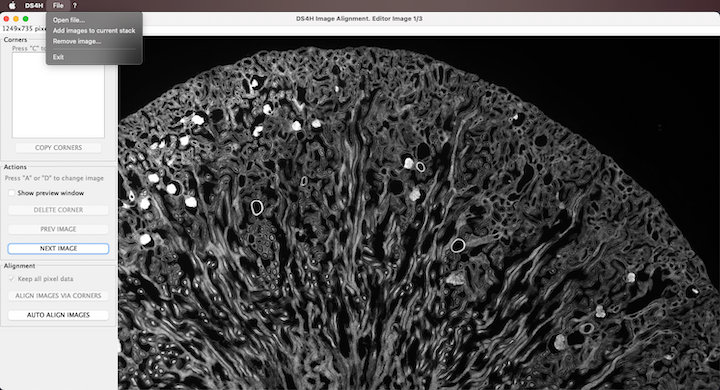
\includegraphics[scale=0.5,keepaspectratio]{windows/menu_principale.png}
    \caption{Schermata principale in cui sono stati aggiunti dei corner points}
    \label{fig:15}
\end{figure}

\subsubsection{Selezione multipla}
\noindent Solo via lista

\subsubsection{Esecuzione Co-registrazione}
\noindent Button + modal scelta
\subsubsection{Salvare Immagine risultante}
\noindent VirtualStack
\subsubsection{Riutilizza Immagine}
\noindent VirtualStack

\subsubsection{Apre Finestra di preview}
\noindent PreviewDialog
\subsubsection{Cmbia immagine di preview}
\noindent PreviewDialog


\subsection{OME Data Model}
\noindent 

  \backmatter{}
  \nocite{*}            % aggiunge tutti i riferimenti nel .bib (anche non citati)
\printbibliography[%  % produce la bibliografia
  heading=bibintoc    % inserisce il titolo nell'indice generale
]

  Ringraziamenti


\end{document}
